\chapter{Casus - Designs}
\label{AppendixDesigns}

De casus bevat een voorgedefinieerde template die exact zal uitgewerkt worden in twee systemen. Beide systemen worden uitgetest op een bestaand design voor een bedrijfswebsite. Deze website bevat de meest typerende en meest belangrijke elementen als voorbeeld voor een CMS.

\begin{figure}[!ht]
  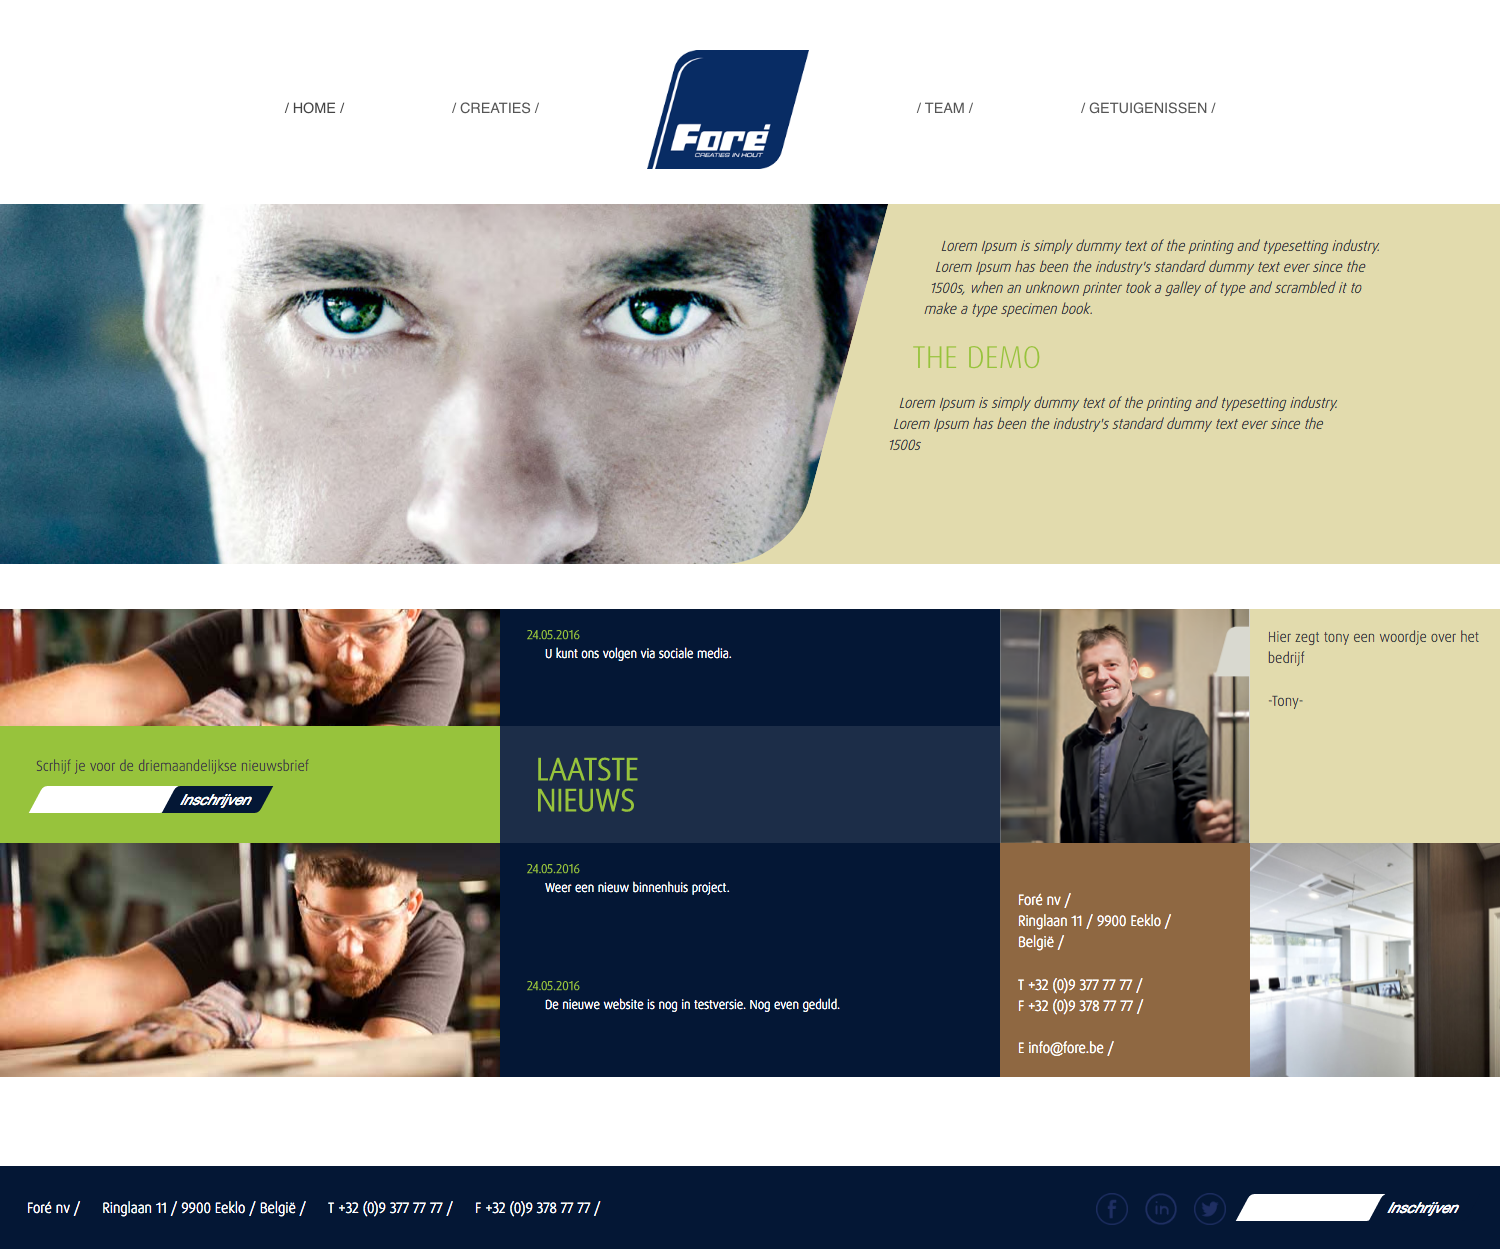
\includegraphics[width=110mm]{img/design-01.png}
  \centering
  \caption{Casus design homepagina}
  \label{fig:Casus design homepagina}
\end{figure}

\begin{figure}[!ht]
  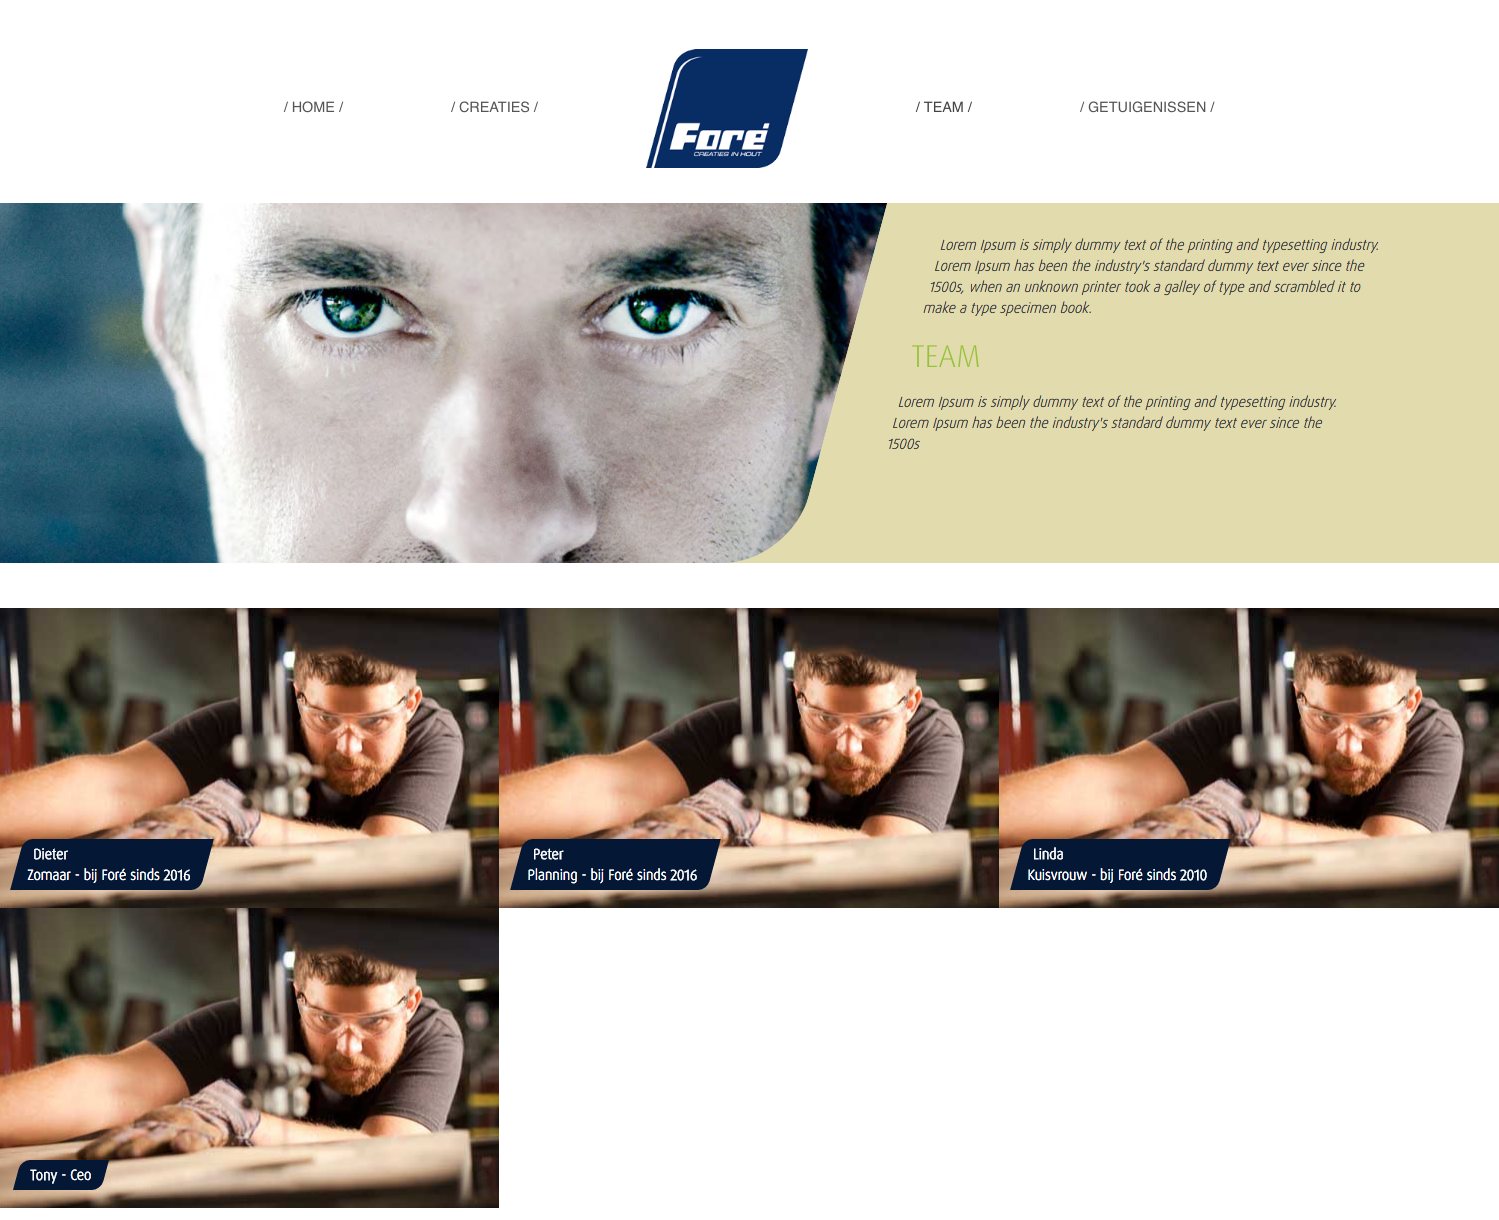
\includegraphics[width=110mm]{img/design-02.png}
  \centering
  \caption{Casus design team}
  \label{fig:Casus design team}
\end{figure}

\begin{figure}[!ht]
  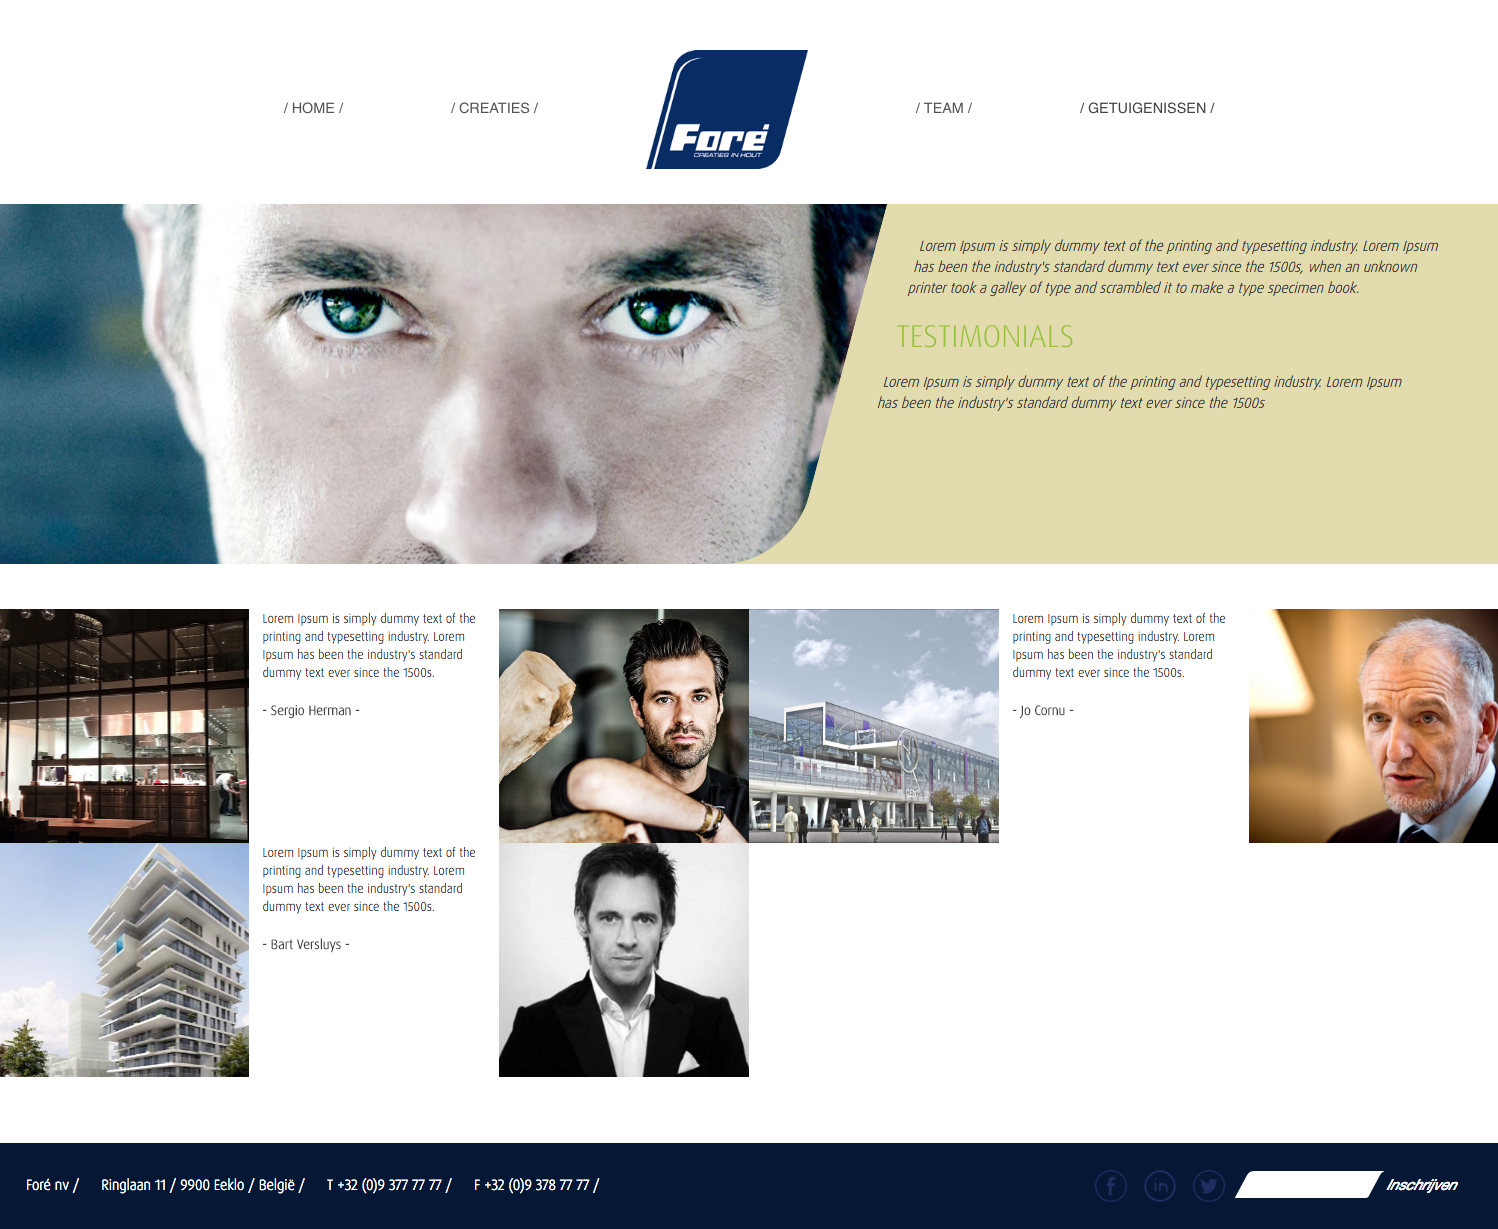
\includegraphics[width=110mm]{img/design-03.png}
  \centering
  \caption{Casus design testimonials}
  \label{fig:Casus design testimonials}
\end{figure}

\begin{figure}[!ht]
  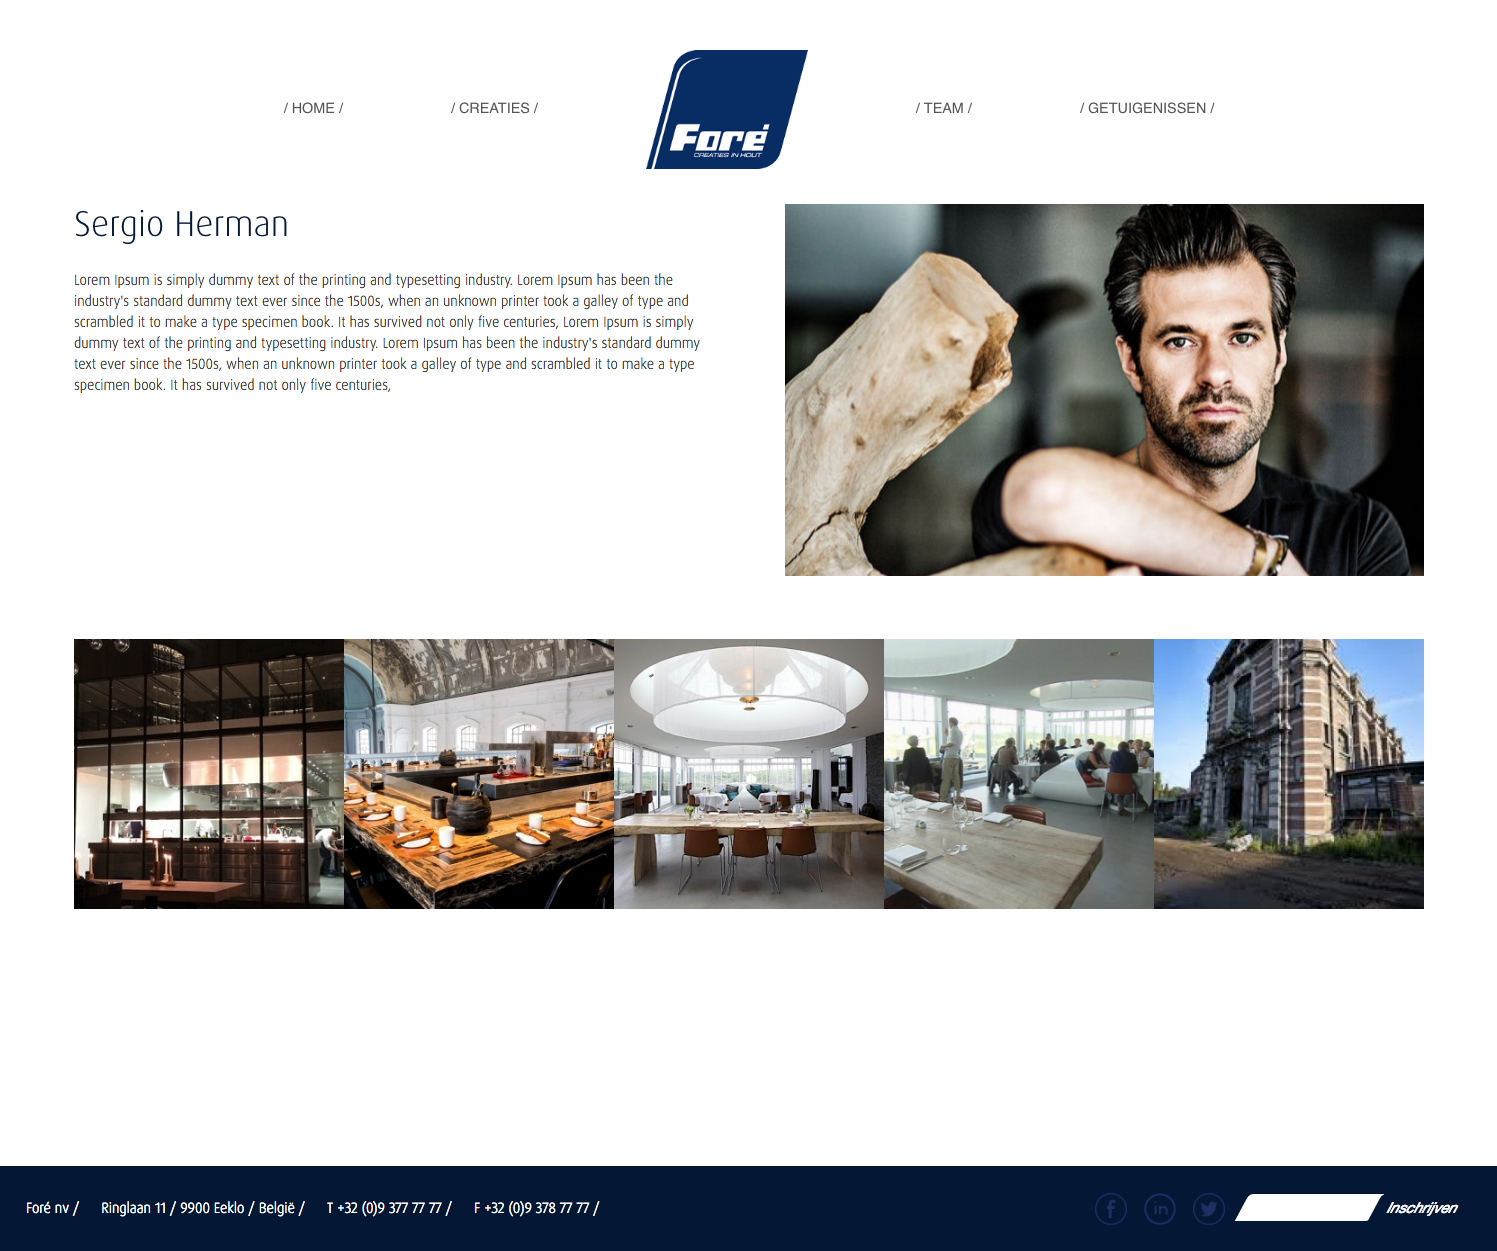
\includegraphics[width=110mm]{img/design-04.png}
  \centering
  \caption{Casus design testimonials detail}
  \label{fig:Casus design testimonials detail}
\end{figure}

\begin{figure}[!ht]
  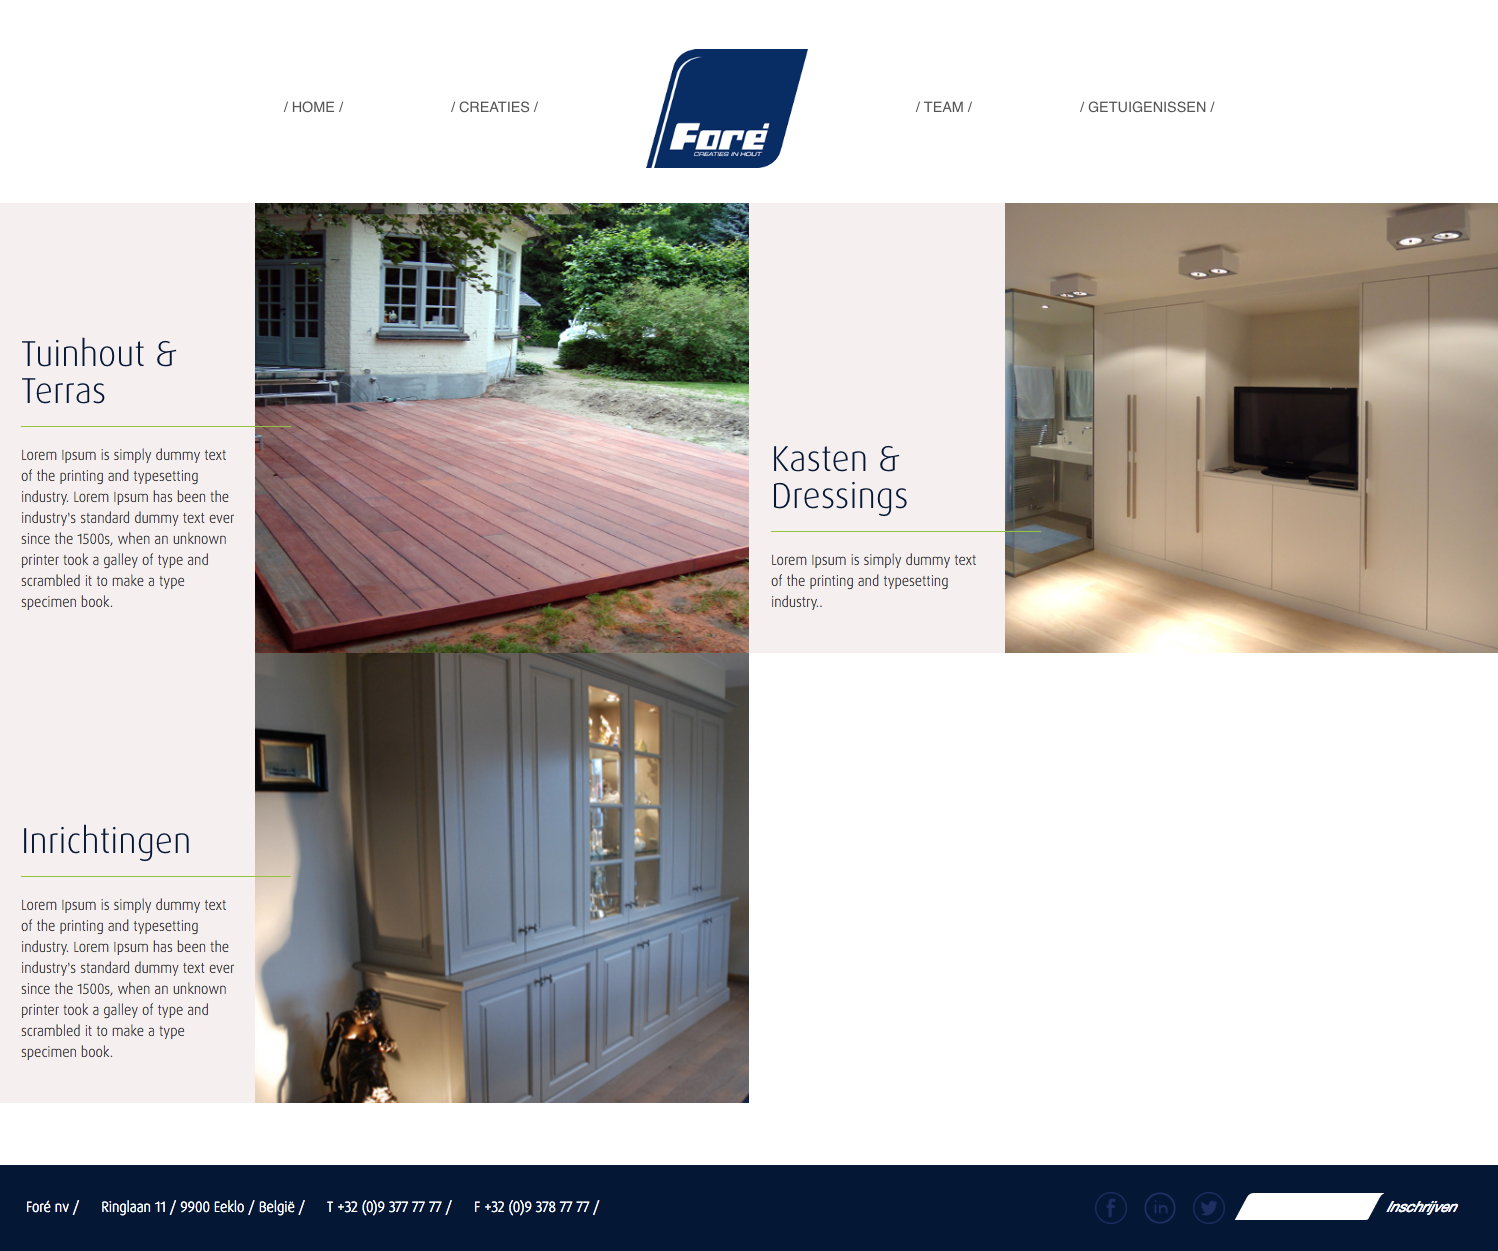
\includegraphics[width=110mm]{img/design-05.png}
  \centering
  \caption{Casus design categorie overzicht}
  \label{fig:Casus design categorie overzicht}
\end{figure}

\begin{figure}[!ht]
  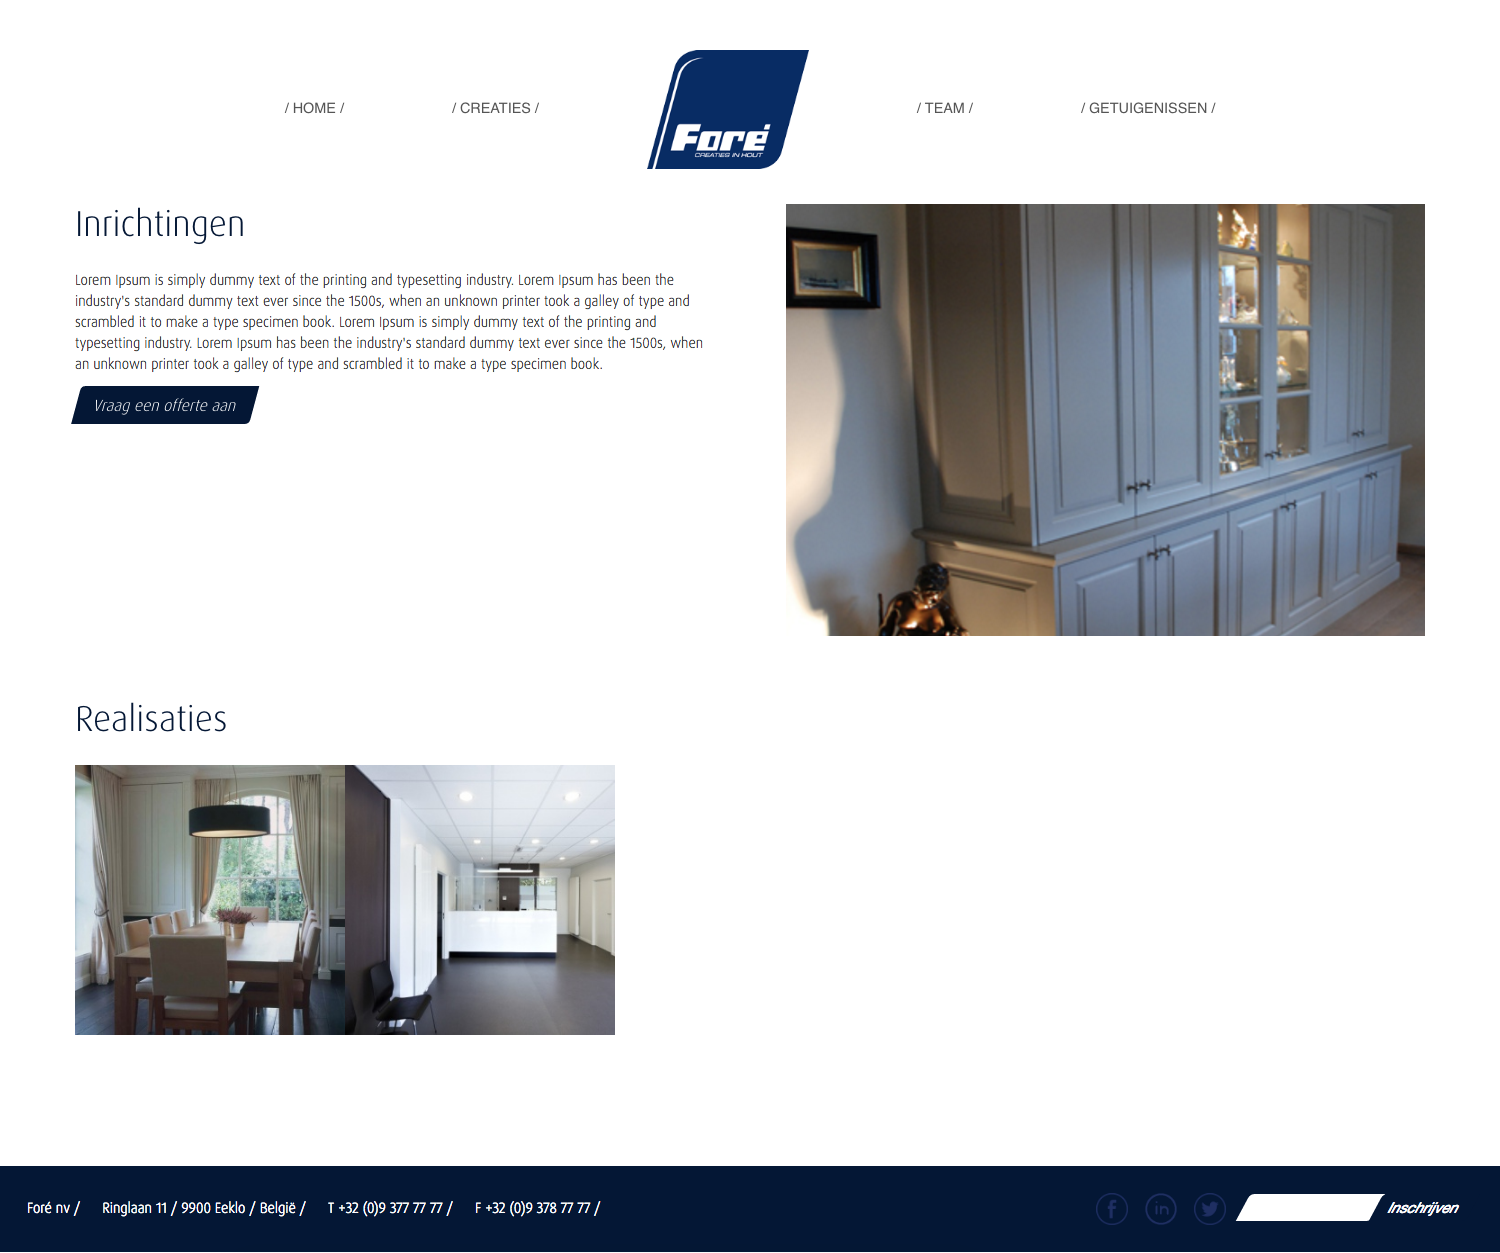
\includegraphics[width=110mm]{img/design-06.png}
  \centering
  \caption{Casus design categorie detail}
  \label{fig:Casus design categorie detail}
\end{figure}

\begin{figure}[!ht]
  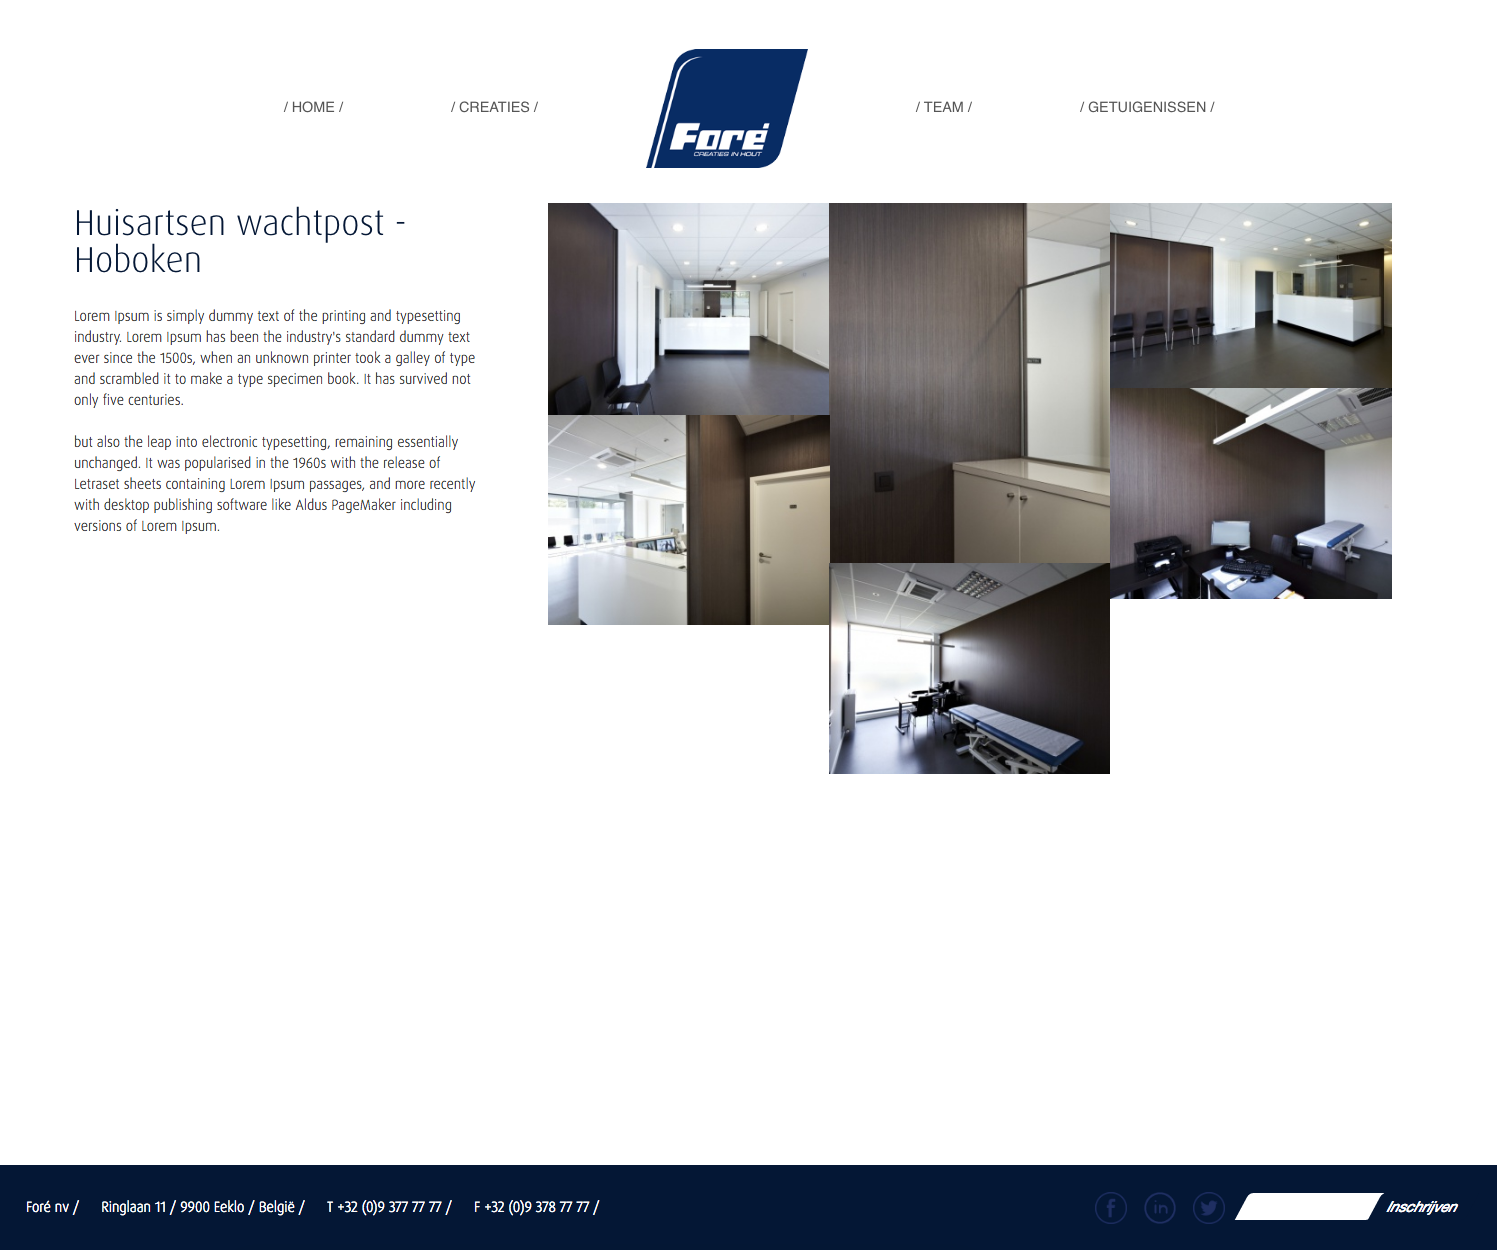
\includegraphics[width=110mm]{img/design-07.png}
  \centering
  \caption{Casus design realisatie}
  \label{fig:Casus design realisatie}
\end{figure}